% !TeX root = responsiveness_tr
% ================================================================
\section{Problem}\label{prresp_Problem}

\begin{figure*}
	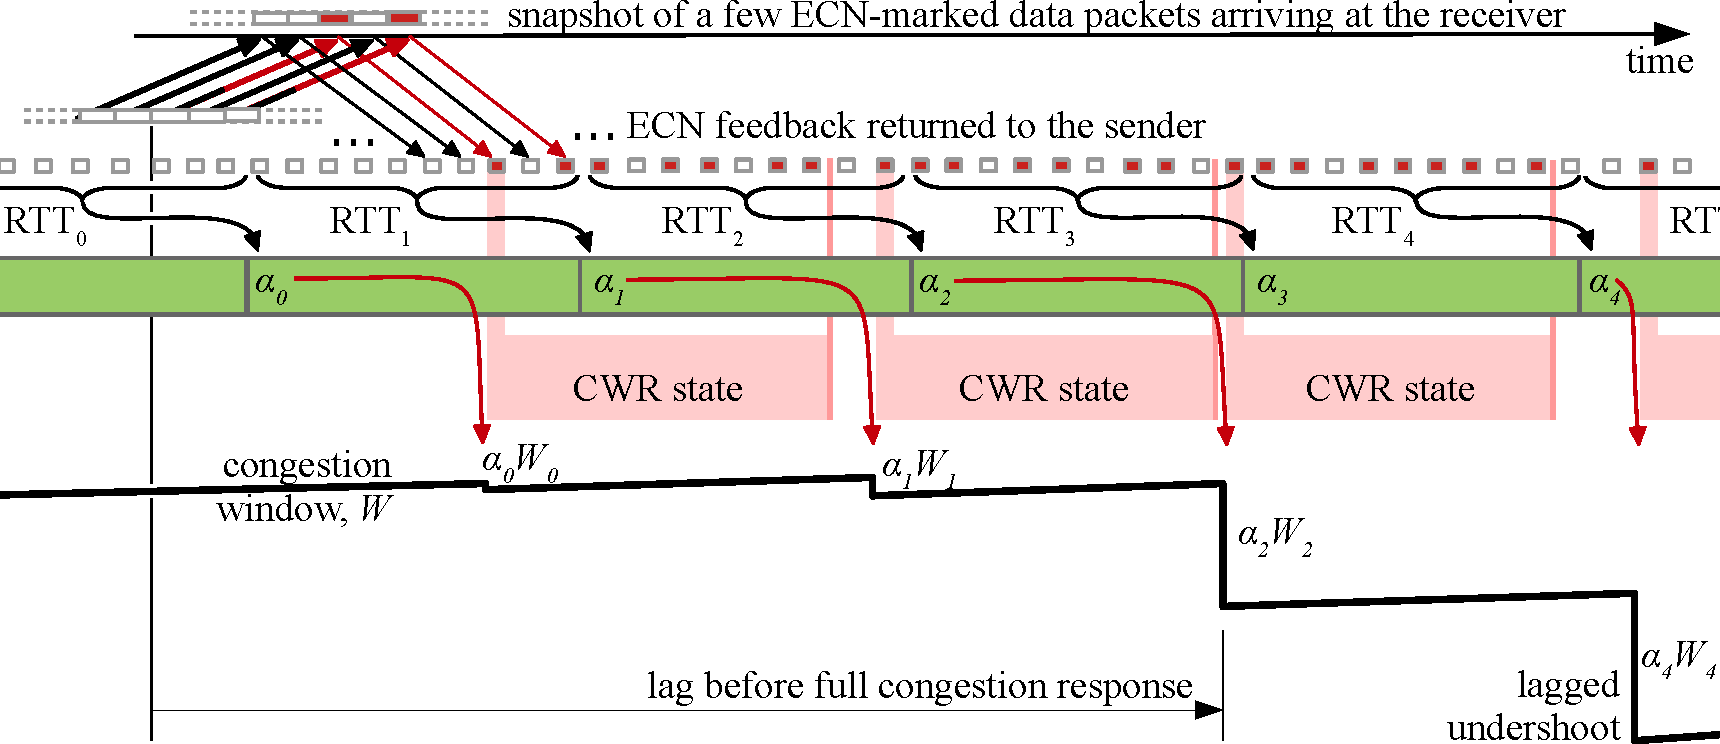
\includegraphics[width=\linewidth]{dctcp-feedback-lag}
	\caption{The problem: DCTCP's two stages for processing congestion feedback: 1) gathering feedback in a fixed sequence of rounds (RTT\(_i\) to calculate the EWMA (\(\alpha_i\)); 2) applying this EWMA on the first feedback mark, when it has had no time to gather enough feedback, which leads to a typically inadequate congestion response before entering congestion window reduced (CWR) state, which suppresses any further response for a round. See text for full commentary.}
	\label{fig:dctcp-feedback-lag}
\end{figure*}

Common implementations of DCTCP~\cite{Alizadeh10:DCTCP} (e.g.\ in Windows, Linux, or FreeBSD~\cite{Bensley17:DCTCP}) take two rounds before a change in congestion on the path fully feeds into the moving average that regulates its response. This is on top of the inherent round trip of delay in the feedback loop.

Both extra rounds are due to the two-stage process for maintaining the EWMA then using it to respond to congestion (see \autoref{fig:dctcp-feedback-lag}). The first stage introduces a round of delay (RTT\(_i\)) while it accumulates the marking fraction before it can calculate the EWMA (\(\alpha_i\)), which it passes to the second stage that uses the EWMA to reduce the congestion window (\(W\)) by \(\alpha_i W_i\). The second extra round of delay is because the first stage clocks independently, while the second stage is triggered by the arrival of congestion feedback (a red-coloured ACK).

So it takes two rounds before a full round of the congestion that triggered the start of the second stage has fed through into the EWMA that the first stage passes to the second. This is further exacerbated by entering congestion window reduced (CWR) state as soon as the initial inadequate response has been applied, which suppresses any further response for a round, while all the congestion feedback arrives. Finally, the lagged congestion response overruns by a round, causing undershoot.

The problem seems to boil down to how to update an EWMA of marking probability on a per-packet basis. But, more specifically, the problem is how to ensure that the time constant over which the per-packet EWMA smooths itself keeps to a set number of rounds, even though the number of packets per round varies.

\section{Per-ACK EWMA}\label{prresp_Per-Packet_EWMA}

Instead of the EWMA of the marking probability being upscaled by a constant factor, it is proposed to upscale it by \texttt{flight\_ / gain}, where \texttt{flight\_} is the packets in flight, and \texttt{gain} is a constant (\texttt{gain < 1}). Then, as shown below, the EWMA can be maintained by a single continuous set of repetitive increments or decrements determined on each ACK.

As we shall see, scaling up the EWMA by \texttt{flight\_} enables the repetitive per-packet operations to \emph{implicitly} smooth the EWMA with a characteristic timescale proportionate to the RTT (specifically, \texttt{RTT/gain}).

This contrasts with the two-stage process of accumulating the marking fraction for a round before feeding it into an EWMA that is \emph{explicitly} clocked per round.

The scaled up EWMA is effectively a smoothed count of the number of congestion marks per RTT, but scaled up by the constant \texttt{1/gain}. The number of marks per RTT (\texttt{v}) is related to the marking probability (\texttt{p}) by \texttt{v = p*flight\_}.

Common implementations of DCTCP incorrectly mimic the timing but not the size of a classical congestion control's response. Classical congestion controls suppress any further response for a round because their initial response is large and fixed. On first onset of congestion, it seems wrong for DCTCP to immediately respond with a tiny reduction (based on the previous absence of congestion), then suppress any further response for a round trip. 

So, once we have an EWMA of congestion marks that is updated continually on every ACK, it becomes possible to spread the reduction over the round. Then,  if congestion continues to rise during the round, the EWMA will grow, and the response can pick up this growth as it proceeds.

\paragraph{Definitions of variables}
\begin{description}[nosep]
	\item [\texttt{g}] = \texttt{1/gain}. By default \texttt{g = 16};
	\item [\texttt{g\_shift}] = \texttt{lg(g)};
	\item [\texttt{av\_up}]: EWMA of the marks per round upscaled by \texttt{g}; Alternatively, it might help to think of this as the EWMA of the marking probability (alpha in DCTCP) upscaled by \texttt{g * flight\_}. 
	\item [\texttt{flight\_}]: the number of packets in flight when the marking probablity was fed into the EWMA;
	\item [\texttt{flight}]: the number of packets in flight now;
	\item [\texttt{ce\_fb}] = 1 if ECN packet feedback; 0 otherwise.
\end{description}

\subsection{Intuition}\label{prresp_intuition}

In DCTCP, the EWMA, \texttt{alpha}, is maintained per round trip as follows (in floating point arithmetic):
\begin{verbatim}
    alpha += (F - alpha)/g,
\end{verbatim}
where F is the fraction of marked bytes accumulated over the last round trip.

This can be approximated (see \S\,\ref{prresp_approx}) by repeatedly updating the EWMA on the feedback of every packet, but scaling down each update by the number of packets in that round, \texttt{flight\_}. That is, the following per-packet update:
\begin{verbatim}
    alpha += (ce_fb - alpha) / (flight_*g).
\end{verbatim}

The above per-packet update of the EWMA is roughly equivalent to the following per-packet update of the upscaled EWMA, \texttt{av\_up}:
\begin{verbatim}
    av_up += ce_fb - av_up/(flight_*g).
\end{verbatim}

\subsection{Implementation}\label{prresp_implementation}

\subsubsection{Maintaining the EWMA}

The \texttt{ce\_fb} term can be implemented by adding 1 to \texttt{av\_up} on feedback of each CE-marked packet. If the upscaling of \texttt{av\_up} by \texttt{g} were removed to produce an EWMA of marks per round, this would be equivalent to adding \texttt{1/g} of a mark.

The number of packets acknowledged in the current round is \texttt{flight}. So repeatedly subtracting \texttt{av\_up/(flight\_*g)} on the arrival of every ACK would reduce \texttt{av\_up} by \texttt{av\_up*flight/(flight\_*g)} in a round. This approximates to \texttt{av\_up/g} per round. In integer arithmetic, that can be implemented by \texttt{av\_up/g} decrements of 1. 

%\begin{figure*}
\begin{verbatim}
On_each_ACK'd_packet {
    av_up += ce_fb - repetitive_div_1(
              av_up, flight*g, &av_carry);
}

// Repeated execution outputs true with 
//  frequency proportional to num/denom
bool repetitive_div_1(u32 num, u32 denom, 
                            u32 *carry) {
    *carry += num;
    if (*carry >= denom) {
        *carry -= denom;
        return true;
    }
    return false;
}
\end{verbatim}
%\caption{Per-ACK maintenance of an EWMA of marks per round}
%\label{fig:prresp_per-ack-ewma_av_up}
%\end{figure*}

This is achieved as shown %in \autoref{fig:prresp_per-ack-ewma_av_up} 
in the C-like pseudocode above by the repetitive additions, comparisons and decrements of a variable called \texttt{av\_carry}, which carries forward the remainder between ACKs. 

We have defined the general-purpose function \texttt{repetitive\_div\_1()} for the repetitive division, which will be reused later for maintaining the congestion window as well.

\autoref{fig:per-ack-ewma-verify} compares toy simulations of the above EWMA and the DCTCP EWMA (without changing cwnd). It can be seen that, when whenever marks arrive, the algorithm always moves immediately, whereas DCTCP's EWMA does nothing until the next round trip cycle.
\begin{figure}[h]
	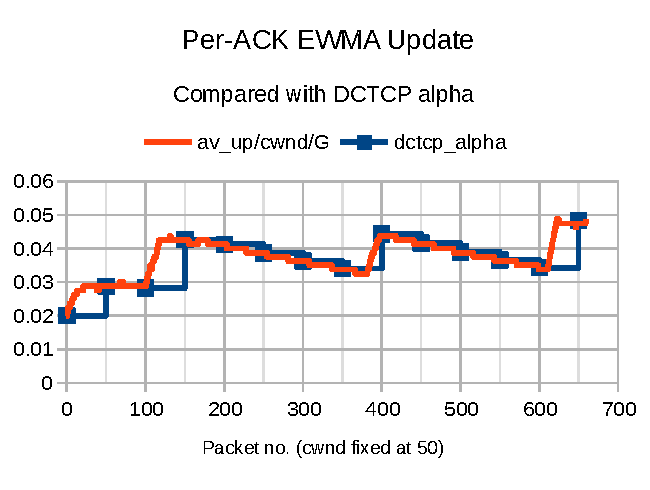
\includegraphics[width=\linewidth]{per-ack-ewma-verify}
	\caption{Initial verification of per-ACK EWMA algorithm, with constant \texttt{cwnd}}\label{fig:per-ack-ewma-verify}
\end{figure}

\subsubsection{Responding to Congestion}\label{prresp_congestion_response}

The approach proposed in this section is not necessarily the final word on how to use the per-ACK EWMA for scalable congestion control (see \S\,\ref{prresp_future} for further ideas). Nonetheless, as a first step, we build incrementally on DCTCP, using its teaching selectively, but not departing too far from its intent. 

DCTCP reduces \texttt{cwnd} by \texttt{alpha*cwnd/2} in any round trip in which CE feedback is present. The proposed approach reduces \texttt{cwnd} by half the average number of marked packets per round, or \texttt{av\_up / (2*g)}. This is broadly equivalent to DCTCP in that it maintains the scalable '\(1/p\)' response function, but with two main quantitative differences:
\begin{itemize}[nosep]
	\item The window reduction is taken as a proportion of what the window has been in recent rounds, not what it is now (as in DCTCP) (see \S\,\ref{prresp_Non-Concerns}).
	\item The window reduction is taken as a proportion of the amount of the window that has been \emph{used} in recent rounds, not the maximum that the flow was entitled to use, i.e.\ packets in flight not \texttt{cwnd}. Thus, if an application-limited flow has only used a quarter of the available window in recent rounds, the proposed reduction of \texttt{cwnd} will be only a quarter of that applied by DCTCP (see \S\,\ref{prresp_Advantage_App-Limited}).
\end{itemize}

The main departure from DCTCP is in the speed of response. Rather than reduce  \texttt{cwnd} on the first sign of CE feedback then suppress further response for a round trip, it is proposed to spread the reduction over the round following the first sign of CE feedback. In other words, use the whole round while in CWR state to reduce \texttt{cwnd} as the EWMA updates, such that, by the end of the round it will still have reduced as much as it would have done if the whole reduction had been applied at the end.

This will exploit the fact that the EWMA (\texttt{av\_up}) is continually updated on every ACK. So, at one extreme, if the first CE mark is immediately followed by many others, the EWMA will rapidly increase early in the round of CWR, and \texttt{cwnd} can be rapidly decreased accordingly. While, at the other extreme, if the first CE mark is the only CE mark in the round, \texttt{cwnd} will still have reduced by \texttt{alpha*cwnd/2} by the end of the round, but the EWMA will hardly have increased above the value it took when the CWR round started.

To spread the reduction over the round, the proposed algorithm above does not divide the round into an arbitrary number of points where \texttt{cwnd} is altered by varying amounts. Instead, it decrements \texttt{cwnd} as soon as the algorithm first calculates that at least one packet of movement is possible. This algorithm would supplant proportional rate reduction (PRR~\cite{IETF_RFC6937:PRR}) when responding to ECN. 

\begin{verbatim}
On_each_ACK'd_packet {
    av_up += ce_fb - repetitive_div_1(
              av_up, flight*g, &av_carry);

    if (!cwr && ce_fb) {
        // Record start of CWR state
        next_seq = snd_next;
        cwr = true;
    }
    if (cwr) {
        // Check still in CWR round
        if (snd_una < next_seq) {
            // Multiplicative Decrease
            cwnd -= repetitive_div_1(
          av_up, flight*g*2, &cwnd_carry);
        } else {
            cwr = false;
        }
    }
}
\end{verbatim}

Details of \texttt{cwnd} processing are omitted from the pseudocode if they are peripheral to the proposed changes. For instance, in real code \texttt{cwnd} would be prevented from falling below a minimum (default 2 segments), and the slow-start threshold would track reductions in \texttt{cwnd} (but see \S\,\ref{prresp_future} for alternative ideas).

Note that \texttt{cwnd} is not updated on the ACK that ends CWR state, because it is updated on the marked ACK that starts CWR state.

As in DCTCP, the EWMA is calculated continuously, but it is only used if there is actual congestion marking, when it is applied for one round of CWR. This is also similar to the approach used to smooth queue measurement in many classical AQMs (e.g.\ PIE, CoDel), where a control law continuously calculates a smoothed likelihood of signalling (drops or marks), but the AQM only emits signals if the actual queue is above a certain threshold, even though it continues to evolve the signalling level.

CWR state takes on a meaning that is nearly the opposite of its classical meaning. It no longer means `congestion window reduced; no further reduction for a round'. Instead it means `congestion window \emph{reduction} in progress during this round'. 

\subsubsection{Additive Increase}\label{prresp_Additive_Increase}

For completeness, the pseudocode below includes a Reno-like additive increase. This is intended for periods when the congestion control is close to its operating point (if it is not, see \S\,\ref{prresp_future}).

Like Reno, DCTCP suspends additive increase during CWR state. However, this has been found to cause unnecessary queue variation. This is because DCTCP-like congestion controls are designed to induce roughly 2 ECN marks per round trip in steady state. So, confining increase to periods that are not meant to happen creates an internal conflict within DCTCP's own design. Then, the algorithm's only escape is to store up enough decrease rounds to make space for a compensating period of increase.

Instead, we continue additive increase regardless of CWR state. In place of suspending additive increase for a whole round, a fractional increase is calculated per-ACK and skipped if an ACK carries congestion feedback. This thins down the additive increase as congestion rises (see \S\,3.1 of \cite{Briscoe17a:CC_Tensions_TR}).

The additive increase stores its remainder in the same \texttt{*cwnd\_carry} variable as the multiplicative decrease. So both numerator and denominator are scaled up so that AI uses the same denominator parameter as MD, otherwise the upscaling of the carry variable would be different.

This also requires the reusable repetitive division function to be modified, to be able to either add or subtract the carry. To avoid ambiguity, we have used a slightly different function name, \texttt{repetitive\_div()}.

\begin{verbatim}
On_each_ACK'd_packet {
    // Update EWMA
    av_up += ce_fb - repetitive_div(false,
            av_up, flight*g, &av_carry);

    if (!ce_fb) {
        // Additive Increase
        cwnd += repetitive_div(false,
          g*2, flight*g*2, &cwnd_carry);
    } else if (!cwr) {
        // Record start of CWR state
        next_seq = snd_next;
        cwr = true;
    }

    if (cwr) {
        // Check still in CWR round
        if (snd_una < next_seq) {
            // Multiplicative Decrease
            cwnd -= repetitive_div(true,
          av_up, flight*g*2, &cwnd_carry);
        } else {
            cwr = false;
        }
    }
}

// Repeated execution outputs true with 
//  frequency proportional to num/denom
// If add is false, flip direction of carry
bool repetitive_div(bool subtract, 
          u32 num, u32 denom, u32 *carry) {
    _outcome = false;
    if (subtract) *carry = denom - *carry;
    *carry += num;
    if (*carry >= denom) {
        *carry -= denom;
        _outcome = true;
    }
    if (subtract) *carry = denom - *carry;
    return _outcome;
}
\end{verbatim}

The new \texttt{repetitive\_div()} function has an additional first boolean parameter \texttt{subtract}. When false, the function behaves no differently to the original \texttt{repetitive\_div\_1()} function. When true, it flips the direction of the number space holding the \texttt{*carry} variable, then flips it back again before terminating. This is preferable to switching between addition and subtraction when altering the carry, which would halve the number space available for the scaled up variables.

\section{(Non-)Concerns}\label{prresp_Non-Concerns}

\subsection{Circular Dependency?}\label{prresp_No_Circular_Dependency}

There seems to be a circular dependency, because \texttt{av\_up} is both upscaled by \texttt{cwnd} then used to update \texttt{cwnd}.

In fact, \texttt{av\_up} is upscaled by what \texttt{cwnd} \emph{was} at the time of each repetitive decrement or increment of \texttt{av\_up}. So  \texttt{av\_up} depends on an implicit exponentially weighted moving average of \texttt{cwnd} with a characteristic smoothing timescale of \texttt{g} round trips. This stabilizes the circular dependency.

\subsection{Advantage to Application Limited Flows?}\label{prresp_Advantage_App-Limited}

The reduction to \texttt{cwnd} is spread over the \texttt{flight} packets in a round of CWR, so each reduction is scaled down by \texttt{flight} in the denominator of the call to \texttt{repetitive\_div()}. This means that the decrease of \texttt{cwnd} is actually by a multiplicative factor of \texttt{flight}, not of \texttt{cwnd}.

If a flow is not application-limited, the two amount to the same thing. But for app-limited flows, \texttt{flight} can be lower than \texttt{cwnd}, so the reduction in \texttt{cwnd} will be lower.

If a flow is only using a fraction of its congestion window, and it is experiencing congestion, it implies that other flow(s) have filled the capacity that the app-limited flow is `entitled' to but not using. Then, it could be argued that the other flows have a higher \texttt{cwnd} than they are `entitled' to, so that the app-limited flow can reduce its `entitlement' (\texttt{cwnd}) less than these other flows in response to congestion.

If this argument is not convincing, the reduction in \texttt{cwnd} could be scaled up by \texttt{cwnd/flight}. However, it is possible that the code is reasonable as it stands.

\section{Evaluation Plan}\label{prresp_Evaluation}

For research purposes, we ought not to introduce two changes at once, without evaluating each separately. Therefore, initially, we ought to use the continually updated EWMA, \texttt{av\_up} to reduce \texttt{cwnd} in the classical way. That is, on the first feedback of a CE mark, reduce \texttt{cwnd} once by \texttt{av\_up/(2*g)}. Then suppress further response for a round (CWR state). This should remove one round of lag (originally spent accumulating the marking fraction), but not the other (reducing cwnd in response to a single mark, then doing nothing for a round while the extent of marking is becoming apparent).

Basic experiments will need to compare how quickly a DCTCP flow in congestion avoidance can reduce in response to a newly arriving flow or a reduction in capacity.

Initially the same gain as DCTCP (1/16) ought to be used. But it is possible that the reason the gain had to be so low was because of the two rounds of built in lag in the algorithm. Therefore, it will be interesting to see if the gain can be increased (from 1/16 to 1/8 or perhaps even 1/2 ought to be tried).

The thinking here is that a fixed amount of lag in a response is not the same as smoothing. Lag applies the same response by later. Smoothing spreads the response out, adding lag to the end of the response, but not to the start. Given every DCTCP flow's response to each change has been lagged by 2 rounds, it is possible that all flows have had to be smoothed more than necessary, in order to prevent the excessively lagged responses from causing over-reactions and oscillations.

It will also be necessary to check performance in the following cases that might expose poor approximations in the algorithm (relative to DCTCP):
\begin{enumerate}
	\item When the packets in flight has been growing for some time;
	\item \ldots{}or shrinking for some time;
	\item When the flow is application limited, with packets in flight varying wildly, rather than tracking the smoother evolution of \texttt{cwnd}.
\end{enumerate}

\bob{Outcome of the evaluation itself to be added here.}

\section{Related Work}\label{prresp_related}

Reducing \texttt{cwnd} by half of \texttt{v} per round trip is similar to Relentless TCP~\cite{Mathis09:Relentless}, which reduces \texttt{cwnd} by half a segment on feedback of each CE-marked packet. The difference is that \texttt{v} is a moving average, so it implements smoothing in the sender, whereas Relentless immediately applies a full congestion response without smoothing, because it is designed for smoothing in the network.

Like DCTCP, the per-ACK congestion response proposed in section 5.2 of \cite{Alizadeh11:DCTCP_Analysis} maintains an EWMA of congestion marking probability, \texttt{alpha}. But it reduces \texttt{cwnd} by half of \texttt{alpha} (in units of packets) on feedback of each ECN mark. This causes jumpiness, because marks tend to be bunched into one round then clear for a few rounds, particularly with step-marking. So, even though this algorithm uses the smoothed EWMA for each reduction, it applies many more reductions in those rounds with more marks. In contrast, the approach proposed in the present paper limits the reduction to \texttt{alpha} within a round trip (as DCTCP itself does). Nonetheless, it removes the round of lag that DCTCP's EWMA uses to accumulate the marking probability, and it spreads the reduction over a round to ensure that it picks up feedback as soon as it arrives.

\section{Ideas for Future Work}\label{prresp_future}

An EWMA of a queue-dependent signal is analogous to an integral controller. It filters out rapid variations in the queue that do not persist, but it also delays any response to variations that do persist. Faster control of dynamics should be possible by adding a proportional element, to create a proportional-integral (PI) controller within the sender's congestion control. It would add an extra reduction (increase) to the congestion window dependent on the rate of increase (reduction) in \texttt{av\_up}.

It would be possible to use the per-ACK EWMA of marks per round (\texttt{av\_up} as a good indicator of whether a flow has lost its closed-loop control signal, for instance because another flow has left the bottleneck, or capacity has suddenly increased. A flow could then switch into a mode where it searches more widely for a new operating point, for instance using paced chirping~\cite[\S\,3]{Misund19a:Paced_Chirping_Linux}. For instance, it could calculate the average distance between marks implied by the EWMA \texttt{av\_up}, then deem that marking had significantly slowed if the number of packets since the last mark exceeded some factor times this distance. Alternatively, it might detect when the EWMA of the marks per round had reduced below some absolute threshold (by definition, the marks per round of a scalable congestion control in steady state should be invariant for any flow rate).
